\documentclass[a4paper]{article}
\usepackage[a4paper,margin=0mm]{geometry}
\usepackage{fontspec}
\usepackage{unicode-math}
\usepackage{tikz}
\usepackage[table]{xcolor}
\usepackage[absolute]{textpos}

\setmainfont{Libertinus Serif}
\setsansfont{Libertinus Sans}
\setmathfont{Libertinus Math}

\definecolor{accent}{HTML}{602785}
\definecolor{badge}{HTML}{B8A0C8}
\definecolor{ink}{HTML}{2A2E30}

\setlength{\TPHorizModule}{1mm}
\setlength{\TPVertModule}{1mm}
\setlength{\parindent}{0pt}
\pagestyle{empty}

\begin{document}
\mbox{}
% small ornament
\begin{textblock*}{210mm}(0mm,104mm)
\centering
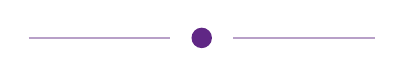
\begin{tikzpicture}
\draw[badge,line width=0.6pt] (-22mm,0) -- (-4mm,0);
\draw[badge,line width=0.6pt] (4mm,0) -- (22mm,0);
\fill[accent] (0,0) circle (1.3mm);
\end{tikzpicture}
\end{textblock*}

\begin{textblock*}{210mm}(0mm,114mm)
\centering
{\sffamily\bfseries\color{accent}\fontsize{12}{14}\selectfont\MakeUppercase{Dedication}}
\end{textblock*}

\begin{textblock*}{130mm}(40mm,128mm)
\centering
{\color{ink}\fontsize{15}{25}\selectfont\itshape
This book series is dedicated to my father,\\[2mm]
{\upshape\bfseries\color{accent}A’zamjonjon Juraboyev,}\\[2mm]
who motivated me to start writing it.\\[8mm]
Although I can’t tell him this,\\
I love him very much.\par}
\end{textblock*}

\begin{textblock*}{210mm}(0mm,196mm)
\centering
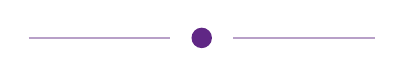
\begin{tikzpicture}
\draw[badge,line width=0.6pt] (-22mm,0) -- (-4mm,0);
\draw[badge,line width=0.6pt] (4mm,0) -- (22mm,0);
\fill[accent] (0,0) circle (1.3mm);
\end{tikzpicture}
\end{textblock*}
\end{document}
